Հայտնի է, որ ոչ բոլոր գրաֆները և մուլտիգրաֆները ունեն միջակայքային ներկումներ: Մուլտիգրաֆների միջակայքային ներկելիության առաջին անհրաժեշտ պայմանը ստացել են Հասրաթյանը և Քամալյանը \cite{AsratianKamalian1994,AsratianKamalian1987}: 
\begin{theorem}
\label{t1_class1} Եթե $G$ մուլտիգրաֆը ունի միջակայքային ներկում, ապա $\chi^{\prime}(G)=\Delta(G)$:
\end{theorem}

Նրանք նաև ցույց են տվել, որ այս պայմանը ոչ միայն անհրաժեշտ, այլև բավարար պայման է համասեռ մուլտիգրաֆների համար:

\begin{theorem}
\label{t1_regular} Եթե $G$-ն համասեռ մուլտիգրաֆ է, ապա
\begin{description}
\item[(1)] $G\in \mathfrak{N}$ այն և միայն այն դեպքում, երբ $\chi^{\prime}(G)=\Delta(G)$,
\item[(2)] Եթե $G\in \mathfrak{N}$ և $w(G)\leq t\leq W(G)$, ապա $G$-ն ունի միջակայքային $t$-ներկում:
\end{description}
\end{theorem}

Այսպիսով, եթե մուլտիգրաֆի քրոմատիկ դասը մեծ է առավելագույն աստիճանից, ապա այն չի կարող լինել միջակայքային ներկելի: Սակայն կան նաև մուլտիգրաֆների այլ ընտանիքներ, որոնք չունեն միջակայքային ներկումներ:

Հաշվարկային դատողություններով կարելի է ցույց տալ, որ որպեսզի մուլտիգրաֆը ունենա միջակայքային ներկում, անհրաժեշտ է, որ մուլտիգրաֆի բոլոր գագաթների աստիճանների ամենամեծ ընդհանուր բաժանարարը հանդիսանա նաև մուլտիգրաֆի կողերի քանակի ընդհանուր բաժանարար:

\begin{theorem}
\label{t1_divisor} Եթե $G$ մուլտիգրաֆի համար գոյություն ունի $d$ թիվ, որը $G$-ի բոլոր գագաթների աստիճանների ընդհանուր բաժանարար է, սակայն $\vert E(G)\vert$-ի բաժանարար չէ, ապա $G\notin \mathfrak{N}$:
\end{theorem}
\begin{proof}[Ապացույց]
Ենթադրենք հակառակը, որ $G$-ն ունի $\alpha$ միջակայքային $t$-ներկում
 որևէ $t\geq \Delta(G)$ թվի համար: $e\in E(G)$ կողը անվանենք
\emph{$d$-կող} եթե $\alpha(e)=d\cdot l$ որևէ $l\in \mathbb{N}$ թվի համար: Քանի որ գոյություն ունի $d$ թիվ այնպես, որ ցանկացած $v\in V(G)$ գագաթի համար $d$-ն $d_{G}(v)$-ի բաժանարար է, իսկ $\alpha$-ն միջակայքային ներկում է, ունենք, որ ցանկացած $v\in V(G)$ գագաթի համար $S\left(v,\alpha\right)$ բազմությունը պարունակում է ճիշտ $\frac{d_{G}(v)}{d}$ $d$-կողեր: $m_{d}$-ով նշանակենք $G$-ում $d$-կողերի քանակը: Էյլերի թեորեմից ստանում ենք, որ
$m_{d}=\frac{1}{2}\sum\limits_{v\in
V(G)}\frac{d_{G}(v)}{d}=\frac{\vert E(G)\vert}{d}$: Ուստի, $d$-ն $\vert E(G)\vert$-ի բաժանարար է, ինչը հակասություն է:
\end{proof}

\begin{corollary}
\label{c1_eulerian} Եթե $G$-ն էյլերյան մուլտիգրաֆ է և $\vert
E(G)\vert$ կենտ է, ապա $G\notin \mathfrak{N}$:
\end{corollary}

Այս հետևանքը առաջին անգամ ստացվել է \cite{Petrosyan2013}-ում:

Կարևոր է նկատել, որ Թեորեմ \ref{t1_divisor}-ի պայմաններին բավարարող գրաֆների դասը ավելի լայն է Հետևանք \ref{c1_eulerian}-ի պայմաններին բավարարող գրաֆների դասից: Մասնավորապես, $K_5$ լրիվ գրաֆը էյլերյան է և ունի զույգ թվով կողեր, սակայն միջակայքային ներկելի չէ համաձայն Թեորեմ \ref{t1_divisor}-ի:
\begin{figure}[h]
\centering
\begin{subfigure}{.5\textwidth}
  \centering
  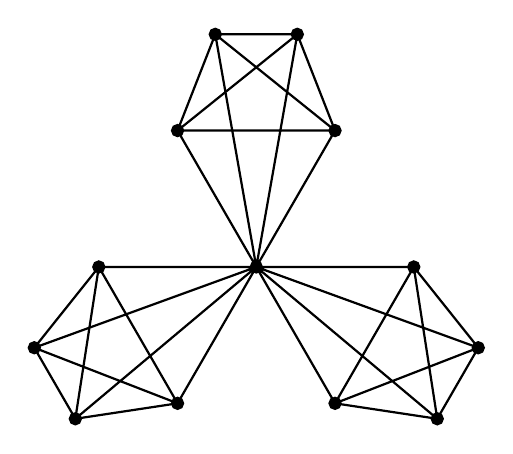
\begin{tikzpicture}[style=thick]
    \coordinate (V0) at (0:0cm);
    \coordinate (V1_1) at (120:2cm);
    \coordinate (V1_2) at (100:3cm);
    \coordinate (V1_3) at (80:3cm);
    \coordinate (V1_4) at (60:2cm);
    \coordinate (V2_1) at (0:2cm);
    \coordinate (V2_2) at (-20:3cm);
    \coordinate (V2_3) at (-40:3cm);
    \coordinate (V2_4) at (-60:2cm);
    \coordinate (V3_1) at (-120:2cm);
    \coordinate (V3_2) at (-140:3cm);
    \coordinate (V3_3) at (-160:3cm);
    \coordinate (V3_4) at (-180:2cm);
    
    \draw (V0) -- (V1_1) -- (V1_3) -- (V0) -- (V1_2) -- (V1_4) -- (V1_1) -- (V1_2) -- (V1_3) -- (V1_4) -- (V0)
    -- (V2_1) -- (V2_3) -- (V0) -- (V2_2) -- (V2_4) -- (V2_1) -- (V2_2) -- (V2_3) -- (V2_4) -- (V0)
    -- (V3_1) -- (V3_3) -- (V0) -- (V3_2) -- (V3_4) -- (V3_1) -- (V3_2) -- (V3_3) -- (V3_4) -- (V0);
    
    \draw[fill=black] (V0) circle (2pt);
    \draw[fill=black] (V1_1) circle (2pt);
    \draw[fill=black] (V1_2) circle (2pt);
    \draw[fill=black] (V1_3) circle (2pt);
    \draw[fill=black] (V1_4) circle (2pt);
    \draw[fill=black] (V2_1) circle (2pt);
    \draw[fill=black] (V2_2) circle (2pt);
    \draw[fill=black] (V2_3) circle (2pt);
    \draw[fill=black] (V2_4) circle (2pt);
    \draw[fill=black] (V3_1) circle (2pt);
    \draw[fill=black] (V3_2) circle (2pt);
    \draw[fill=black] (V3_3) circle (2pt);
    \draw[fill=black] (V3_4) circle (2pt);
 \end{tikzpicture}

  \caption{}
  \label{f1_three_K5s}
\end{subfigure}%
\begin{subfigure}{.5\textwidth}
  \centering
  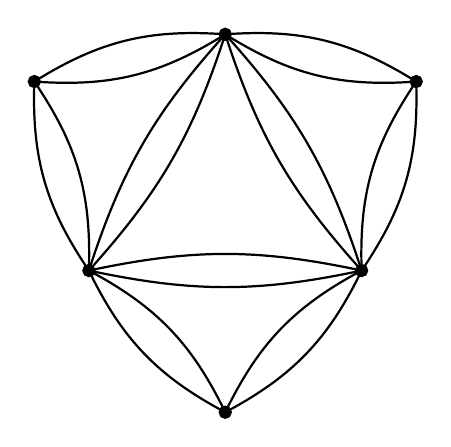
\begin{tikzpicture}[style=thick]
    \coordinate (V1) at (90:2cm);
    \coordinate (V2) at (-150:2cm);
    \coordinate (V3) at (-30:2cm);
    \coordinate (V12) at (150:2.8cm);
    \coordinate (V13) at (30:2.8cm);
    \coordinate (V23) at (-90:2.8cm);
    
    \draw (V1) edge[bend left=18] (V13);
    \draw (V1) edge[bend left=-18] (V13);
    \draw (V1) edge[bend left=18] (V12);
    \draw (V1) edge[bend left=-18] (V12);
    \draw (V1) edge[bend left=12] (V3);
    \draw (V1) edge[bend left=-12] (V3);
    \draw (V1) edge[bend left=12] (V2);
    \draw (V1) edge[bend left=-12] (V2);
    
    \draw (V2) edge[bend left=18] (V23);
    \draw (V2) edge[bend left=-18] (V23);
    \draw (V2) edge[bend left=18] (V12);
    \draw (V2) edge[bend left=-18] (V12);
    \draw (V2) edge[bend left=12] (V3);
    \draw (V2) edge[bend left=-12] (V3);
    
    \draw (V3) edge[bend left=18] (V23);
    \draw (V3) edge[bend left=-18] (V23);
    \draw (V3) edge[bend left=18] (V13);
    \draw (V3) edge[bend left=-18] (V13);
    
    \draw[fill=black] (V1) circle (2pt);
    \draw[fill=black] (V2) circle (2pt);
    \draw[fill=black] (V3) circle (2pt);
    \draw[fill=black] (V12) circle (2pt);
    \draw[fill=black] (V13) circle (2pt);
    \draw[fill=black] (V23) circle (2pt);
 \end{tikzpicture}
  
  \caption{}
  \label{f1_multi}
\end{subfigure}
\caption{Միջակայքային ներկում չունեցող մուլտիգրաֆների օրինակներ, որոնք բավարարում են Թեորեմ \ref{t1_class1}-ի անհրաժեշտ պայմանին, սակայն չեն բավարարում Թեորեմ \ref{t1_divisor}-ի անհրաժեշտ պայմանին:}
\end{figure}
Հարկ է նշել, որ Թեորեմ \ref{t1_divisor}-ի անհրաժեշտ պայմանը չի հանդիսանում Թեորեմ \ref{t1_class1}-ի մասնավոր դեպք: Դիտարկենք Նկ. \ref{f1_three_K5s}-ում պատկերված գրաֆը, որը ստացվում է երեք օրինակ $K_5$ գրաֆներից մեկական գագաթ նույնացնելով: Այս գրաֆի առավելագույն աստիճան ունեցող գագաթը միակն է, ուստի, համաձայն Վիզինգի հայտնի թեորեմի (\cite{Vizing1965critical}), նրա քրոմատիկ դասը հավասար է առավելագույն աստիճանին: Մյուս կողմից՝ այն ունի 30 կող, իսկ բոլոր գագաթների աստիճանները բաժանվում են չորսի, հետևաբար այն չունի միջակայքային ներկում ըստ Թեորեմ \ref{t1_divisor}-ի: Գոյություն ունեն այսպիսի հատկություններով անվերջ թվով մուլտիգրաֆներ: Մասնավորապես, եթե վերցնենք կամայական էյլերյան մուլտիգրաֆ $G$, որի համար $\chi'(G)=\Delta(G)$, և բոլոր կողերի պատիկությունը մեծացնենք $2r$ անգամ ($r \in \mathbb{N}$), ապա ստացված էյլերյան մուլտիգրաֆը կունենա զույգ թվով կողեր, կունենա ճիշտ կողային ներկում առավելագույն աստիճանին հավասար գույներով, սակայն չի ունենա միջակայքային ներկում ըստ Թեորեմ \ref{t1_divisor}-ի (Նկ. \ref{f1_multi}):

